\begin{figure*}[tp]
    \centering
    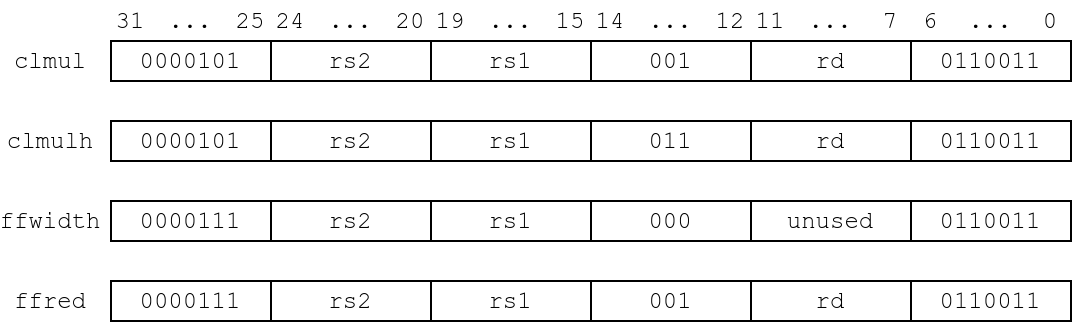
\includegraphics[width=0.8\linewidth]{img/instr.png}
    \caption{The instruction format for the custom galois field arithmetic instructions.}
    \Description{The instruction format for the custom galois field arithmetic instructions.}
    \label{fig:instr}
\end{figure*}

This section describes the ISA extension for RISC-V processors proposed in this work. The selection criteria
of the opcodes were based on the SweRV-EL2 \cite{marena2019risc} microarchitecture. 

The operation added in this extension is the multiplication of finite fields since the sum of two numbers in 
$GF(2^m)$ is only an XOR operation, and it is already defined in RV32I / RV64I. The multiplication is done in three different 
instructions (See Section \ref{section:gf_mult}): carry-less multiplication (CLMULH and CLMUL) and polynomial reduction (FFRED).

To correctly multiply two numbers in $GF(2^m)$, it is also necessary to indicate the irreducible polynomial and the polynomial 
degree to the processor. Therefore, additional instruction is required to pass these parameters (FFWIDTH).

In some processors, such as SweRV-EL2, carry-less multiplication is already implemented in the processor as an extension. Hence, 
the opcode is kept for a compatibility and resource sharing issue.

We decided not to implement the square function and the inverse of $GF(2^m)$ since they are modules that require much logic 
and can also be calculated using finite field multiplication. In more specific computers, these two instructions can be added to 
improve the system's efficiency at the expense of increasing logic utilization.

Figure \ref{fig:instr} shows the formats of the custom instructions proposed in this work. As we can see here, the carry-less multiplication 
keeps the RISC-V extension B format. 

The parameters that receive and return the instructions are:

\begin{itemize}
    \item \textbf{FFWIDTH}: It receives in RS1 the degree of the polynomials, and in RS2, the irreducible polynomial. Since RISC-V registers are 32-bits, 
    the most significant bit of the irreducible polynomial is assumed to be logical 1 when the degree of the input polynomials is 32. For example, for AES, 
    the polynomial degree (RS1) is 8, and the irreducible polynomial (RS2) is 0x11B.
    \item \textbf{FFRED}: It receives the polynomial to be reduced as parameters. In RS1, it receives the high part, and in RS2, the low part of the polynomial. 
    This instruction returns the reduced polynomial $c(x)$. 
    \item \textbf{CLMULH \& CLMUL}: The parameters are the same as extension B.
\end{itemize}

\begin{lstlisting}[caption={GF multiplication for AES},captionpos=b,label={lst:aes}]
li	    a5, 8       % Polynomial degree
li	    a4,283      % Irreducible polynomial
ffwidth	a5,a5,a4    % Load the parameters
...
lbu	    a4,0(a0)
lbu	    a7,0(a1)
clmul	a4,a4,a7    % CL multiplication
li	    a5,0
ffred	a7,a5,a4    % Polynomial reduction
\end{lstlisting}

An example of the multiplication of finite fields using the custom instructions is shown in Listing \ref{lst:aes}. 
This example is a part of the AES code. The FFWIDTH instruction appears only for the first time to tell the hardware 
the polynomial degree and the irreducible polynomial. 
The register RS1 passed to FFRED is 0 because AES uses polynomials that belong to $GF(2^8)$ 
and the bits 63-32 will always be zero after carry-less multiplication.

